\documentclass[11pt]{article}

\author{Math 106}
\date{Due Friday, Oct 13 by 11:59pm} 
\title{Homework 5}

\usepackage{graphicx,xypic}
\usepackage{amsthm}
\usepackage{amsmath,amssymb}
\usepackage{amsfonts}
\usepackage{xcolor}
\usepackage[margin=1in]{geometry}
\usepackage[shortlabels]{enumitem}
\newtheorem{problem}{Problem}
\renewcommand*{\proofname}{{\color{blue}Solution}}


\setlength{\parindent}{0pt}
\setlength{\parskip}{1.25ex}


\begin{document}

\maketitle

% You are required to put your name here:
{\bf\Large Name:} 


\vspace{.3in}
Topics covered: first fundamental form, area, Gauss map

Instructions: 
\begin{itemize}
\item This assignment must be submitted on Gradescope by the due date. 
\item If you collaborate with other students (which is encouraged!), please mention this near the corresponding problems. 
\item If you are stuck, please ask for help (from me, a TA, a classmate). Use ed discussions!  
\item You may freely use any fact proved in class. In general, you should provide proof for facts used that were not proved in class. 
\item Please restrict your solution to each problem to a single page. Usually solutions can be even shorter than that. If your solution is very long, you should think more about how to express it concisely.
\end{itemize}
\pagebreak 





\begin{problem}
Compute the first fundamental forms of the ellipsoid 
\[\phi(u,v)=(a\sin u\cos v,b\sin u\sin v,c\cos u)\]
where $a,b,c$ are positive constants.
\end{problem}

\begin{proof}

\end{proof}

\pagebreak

\begin{problem}
Derive a general formula for the area of a surface of revolution (say, of a curve in the $xz$-plane, revolving about the $z$-axis) by finding a chart and computing the first fundamental form.\footnote{Perhaps you did this some other way in MVC.} Use this to compute the area of the torus surface from class. 
\end{problem}

\begin{proof}

\end{proof}

\pagebreak


\begin{problem}
Consider the following parameterization of the M\"obius band.\footnote{Remark: you probably found a similar parameterization on last week's homework.} 
\[\phi(t,\theta)=\big(
(2+t\cos(\theta/2))\cos\theta, 
(2+t\cos(\theta/2))\sin\theta, 
t\sin(\theta/2)
\big)\>\>\>\>\>t\in[-1,1],\theta\in[0,2\pi]\]
Use this to compute the area of the M\"obius band.\footnote{Aside: why does the area make sense?? The M\"obius band does not have a unit normal!}  \footnote{Encouragement: the computation gets complicated, but it should simplify (have faith!).}
\end{problem}

\begin{proof}

\end{proof}

\pagebreak


\begin{problem}
Describe the image of the Gauss map of the following surfaces. Do \underline{not} compute using a chart -- there is an easier way to reason.
\begin{enumerate}[(a)]
\item paraboloid $z=x^2+y^2$ 
\item hyperboloid $x^2+y^2-z^2=1$
\end{enumerate} 
\end{problem}

\begin{proof}

\end{proof}

\pagebreak

\begin{problem}
In this problem you prove the spectral theorem for self-adjoint linear operators of $\mathbb R^2$. \footnote{Remark: This special case of the theorem is the most important case for us in the course.}

Fix a self-adjoint linear map $A:\mathbb R^2\to\mathbb R^2$. Consider the function $f:\mathbb R^2\to\mathbb R$ defined by $f(p)=A(p)\cdot p$ and let $\alpha:[0,2\pi]\to\mathbb R^2$ denote the standard parameterization of the unit circle. 
\begin{enumerate}[(a)]
\item Compute $(f\circ\alpha)'(t)$ and prove that $t$ is a critical point of $f\circ\alpha$ if and only if $\alpha(t)$ is an eigenvector of $A$. Relate the corresponding eigenvalue to $f$. \footnote{Recall: A critical point of a function $g:\mathbb R\to\mathbb R$ is a value $t$ so that $g'(t)=0$. An eigenvalue of a linear operator $A$ is a nonzero vector $w$ so that $Aw=cw$ for some scalar $c$.}
\item Use facts from calculus to deduce that either $A$ is a scalar matrix or $A$ has two distinct eigenvalues. 
\item Prove that there exist a pair of eigenvectors for $A$ that form an orthonormal basis for $\mathbb R^2$. \footnote{Hint: this is just a linear algebra exercise. Make sure to use the hypothesis...}
\end{enumerate} 
\end{problem}

\begin{proof}

\end{proof}

\pagebreak

\begin{problem}[Bonus]
A linkage is a collection of rods in the plane. The following picture shows two different linkages. 
\begin{center}
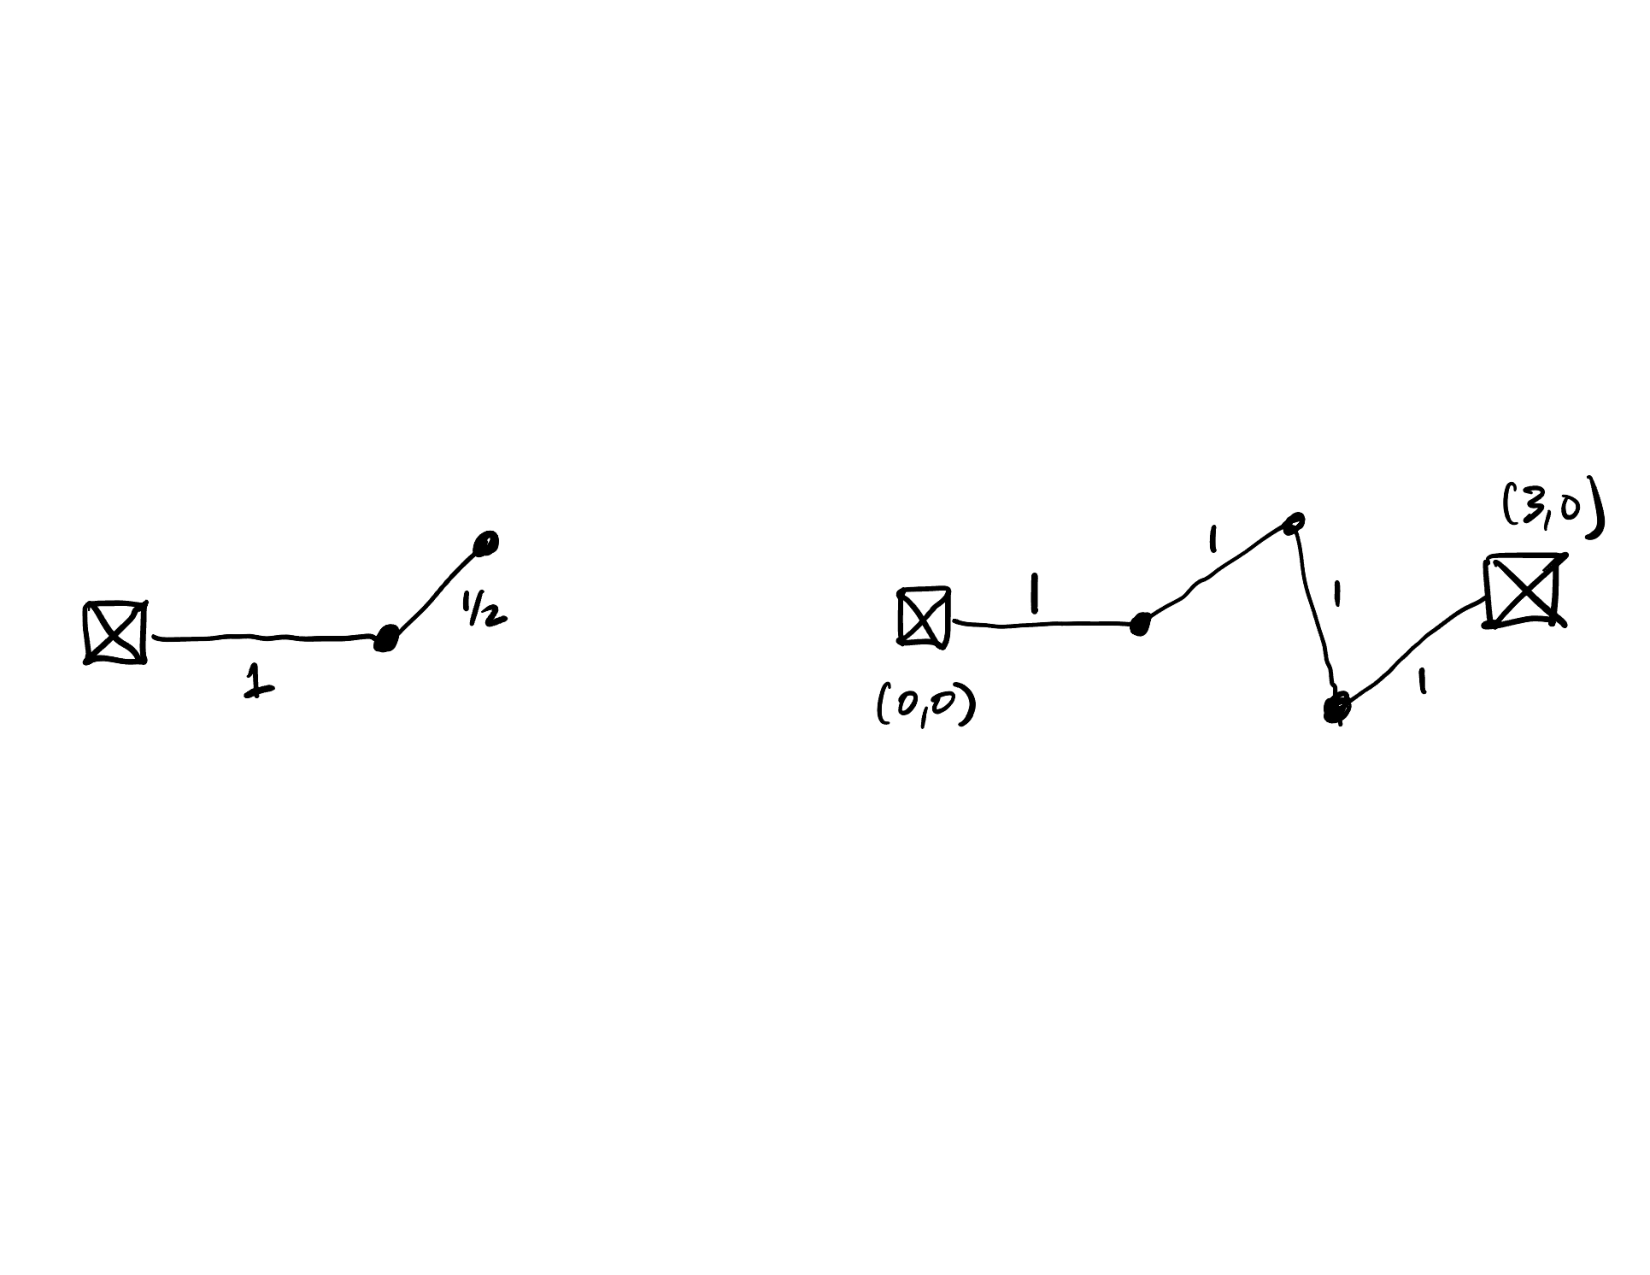
\includegraphics[scale=.4]{linkage}
\end{center}
The configuration space of a linkage is the set of all possible positions of the joints of the rods (this is a subset of some Euclidean space). The configuration space of the two linkages above are surfaces. Identify these surfaces. 
\end{problem}

\begin{proof}

\end{proof}


\end{document}